\begin{appendices}
\section{Erstellung der Datenbank}
%TODO: Name aus Termin-Tabelle nehmen
\lstinputlisting[language=sql, caption={Erstellung der DB}, label=lst:promise]{code/SteckerbotDBModelcreate.sql}
\section{Anwendungsfalldiagramme}
\label{sec:usecase-diagram}

\begin{figure}[htbp]
    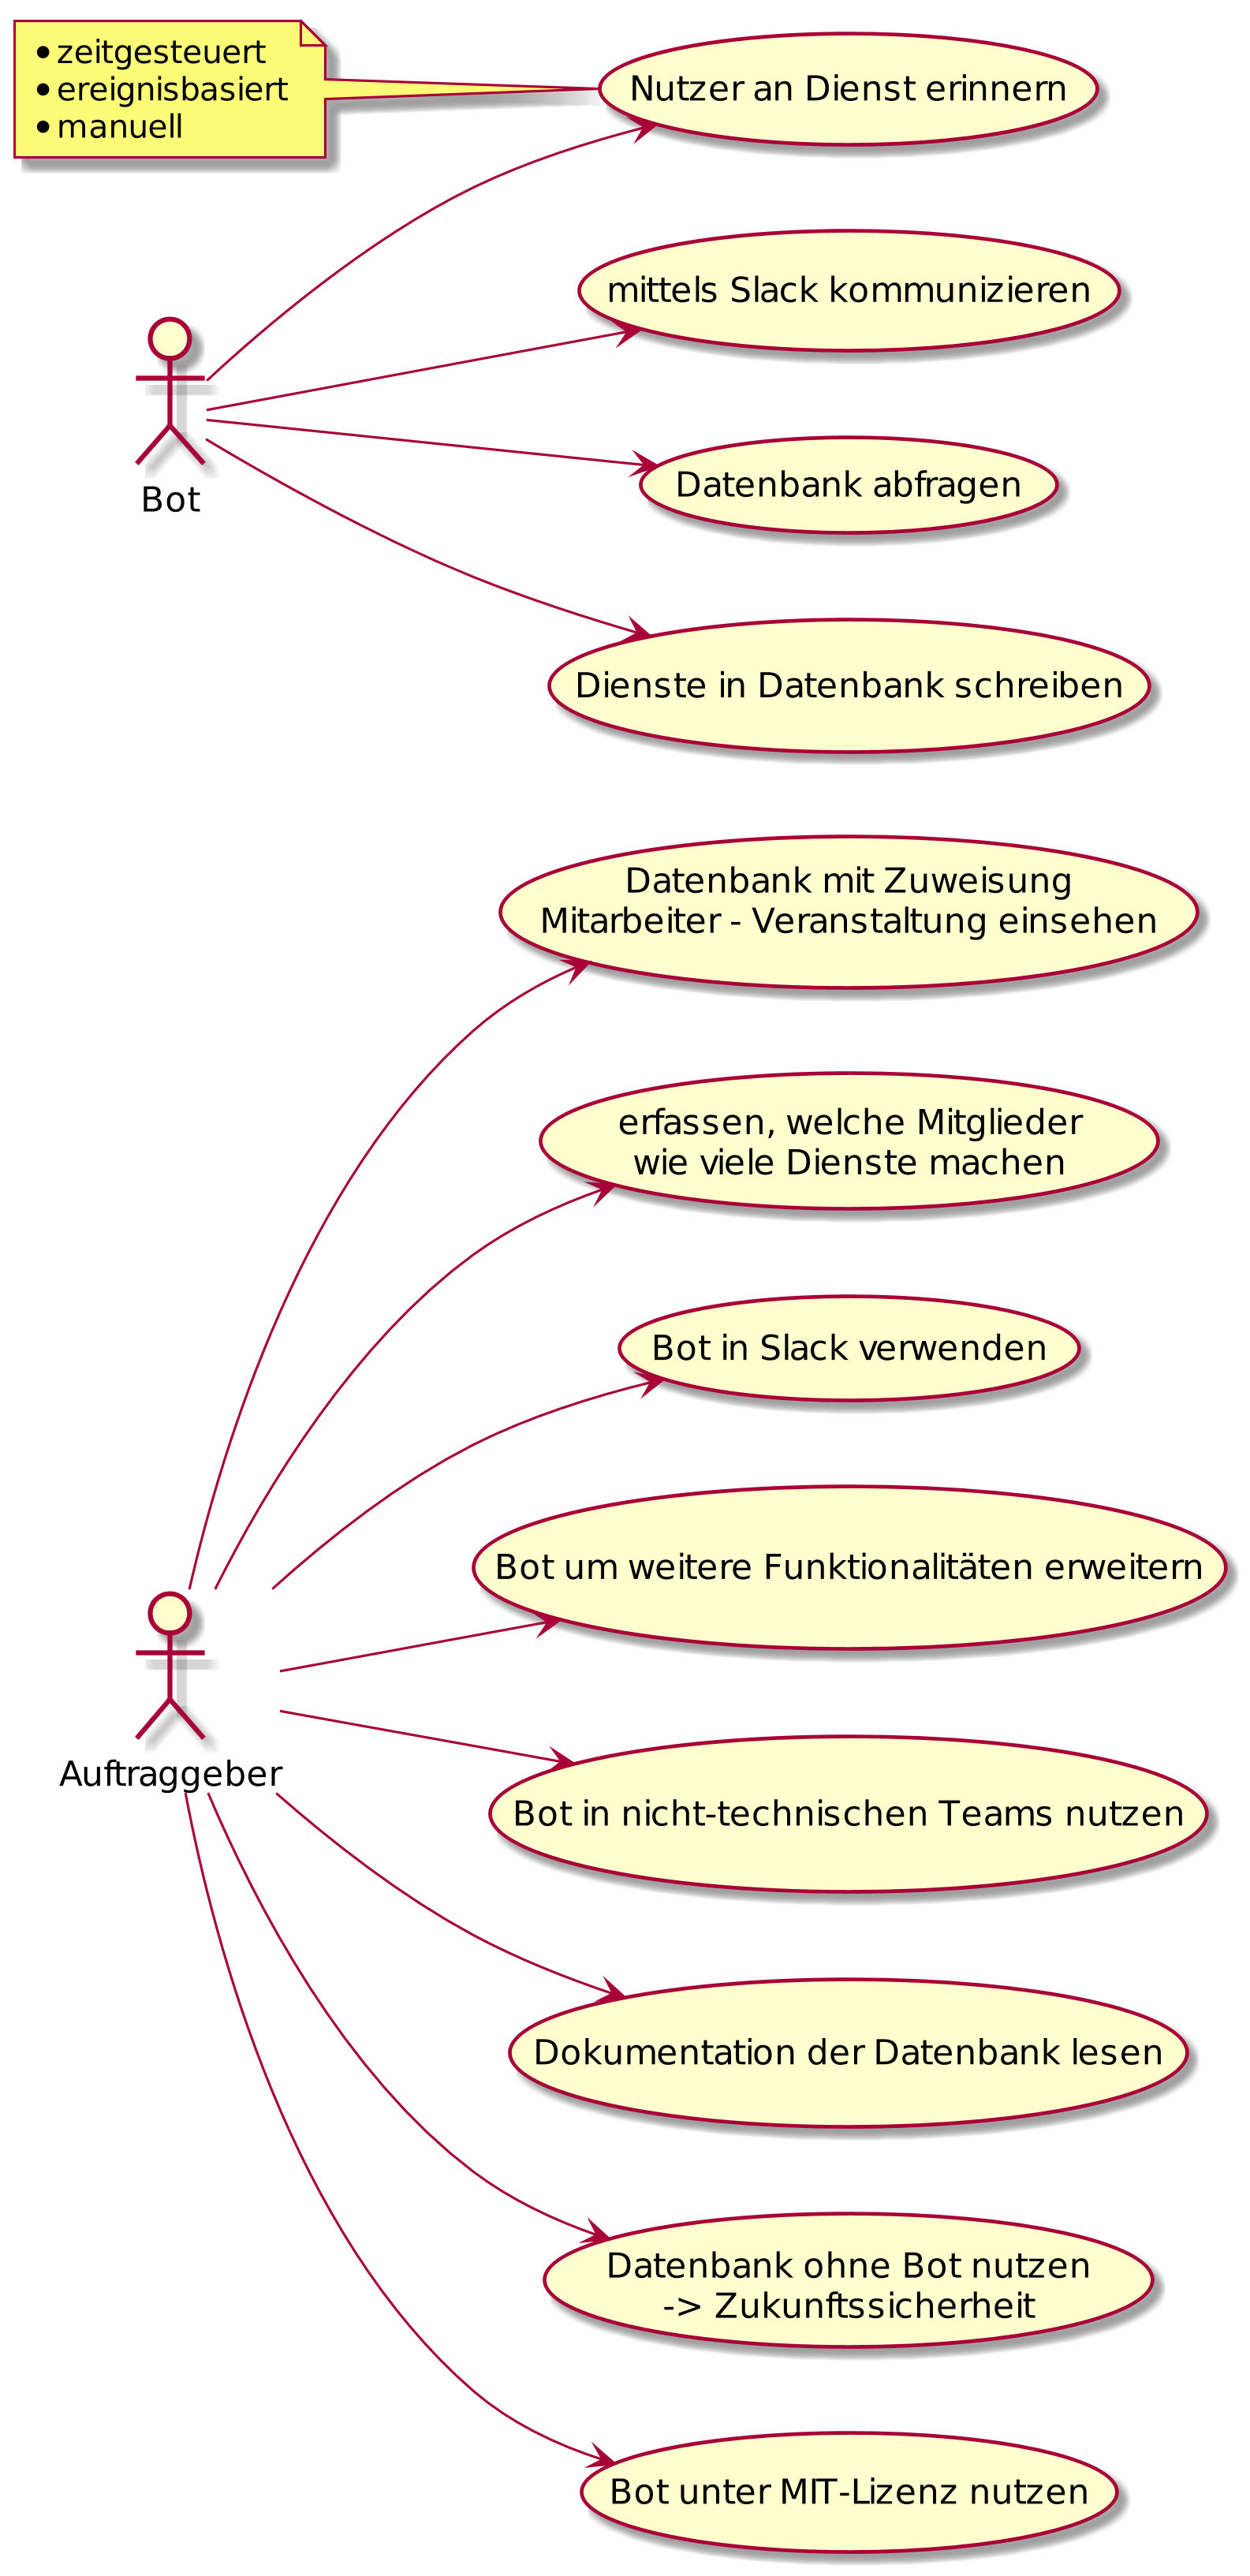
\includegraphics[width=0.7\textwidth]{../docs/uml/usecase-stakeholder.png}
    \caption{Anwendungsfalldiagramm für Auftraggeber und Bot}
    \label{img:usecase-auftrag}
\end{figure}

\begin{figure}[htbp]
    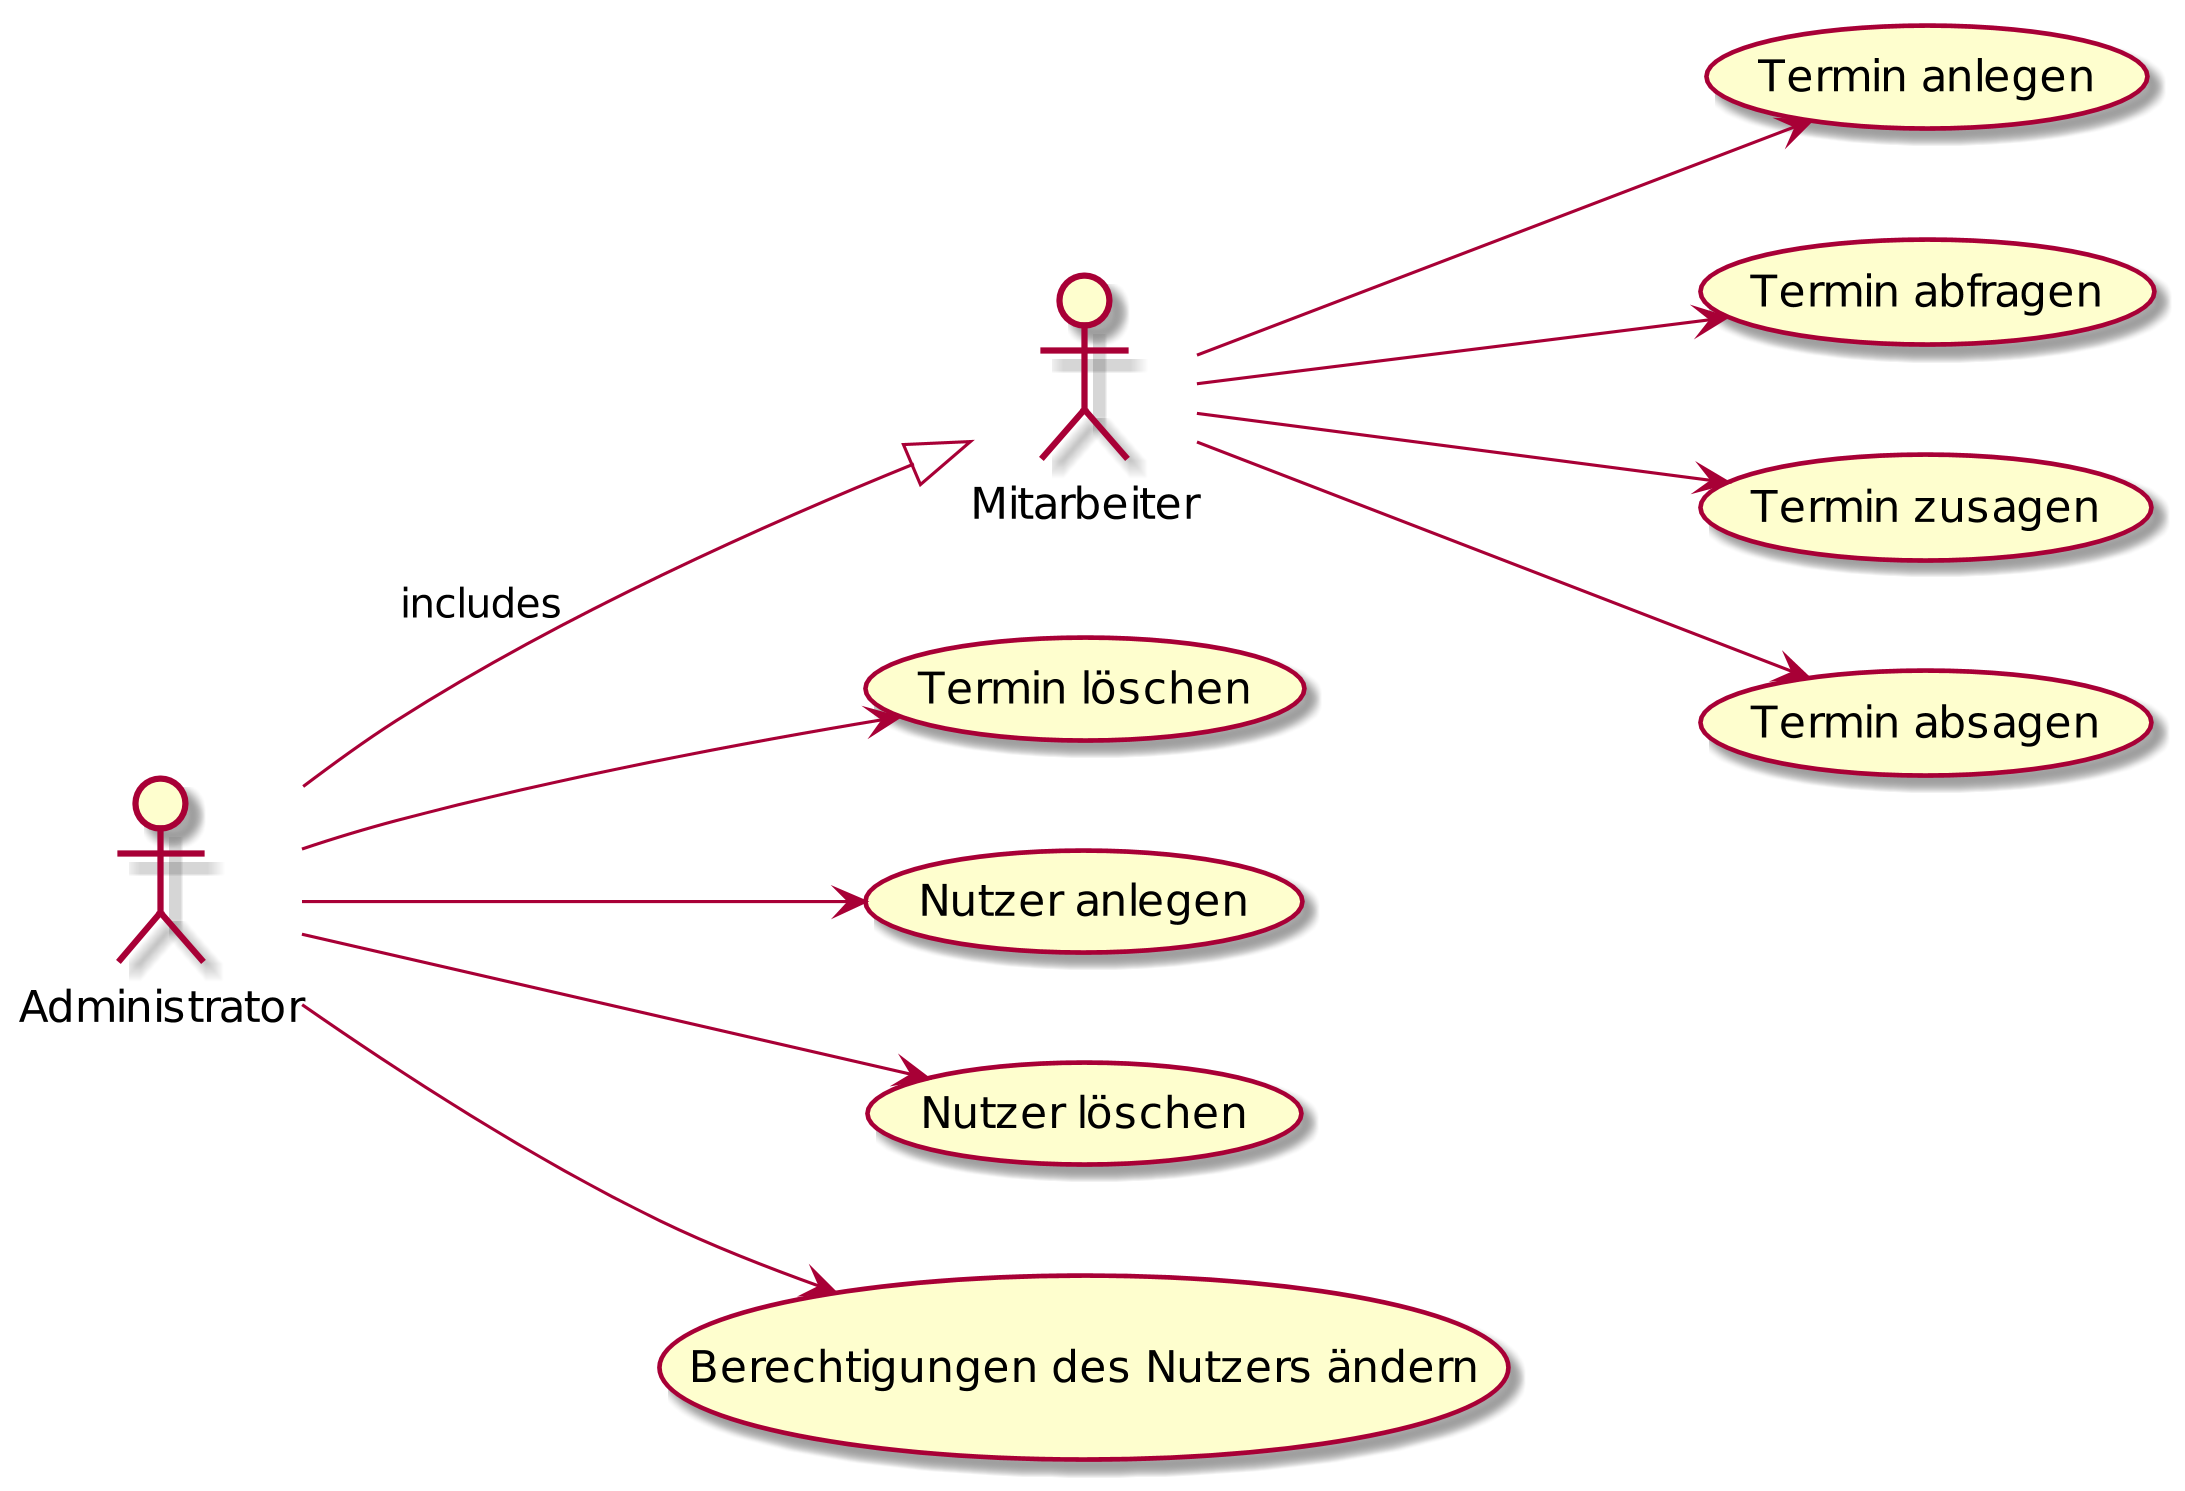
\includegraphics[width=0.9\textwidth]{../docs/uml/usecase-berechtigung.png}
    \caption{Anwendungsfalldiagramm zur Abgrenzung von Mitarbeiter und Administrator}
    \label{img:usecase-berechtigung}
\end{figure}

\section{Docker-Umgebung}
\lstinputlisting[language=bash, caption={Dockerfile für Hubot}, label=lst:dockerfile]{code/Dockerfile}
\lstinputlisting[language=yaml, caption={docker-compose.yml}, label=lst:docker-compose]{code/docker-compose.yml}

% \todo{Projektplan dazu?}
\section{Projektplan}
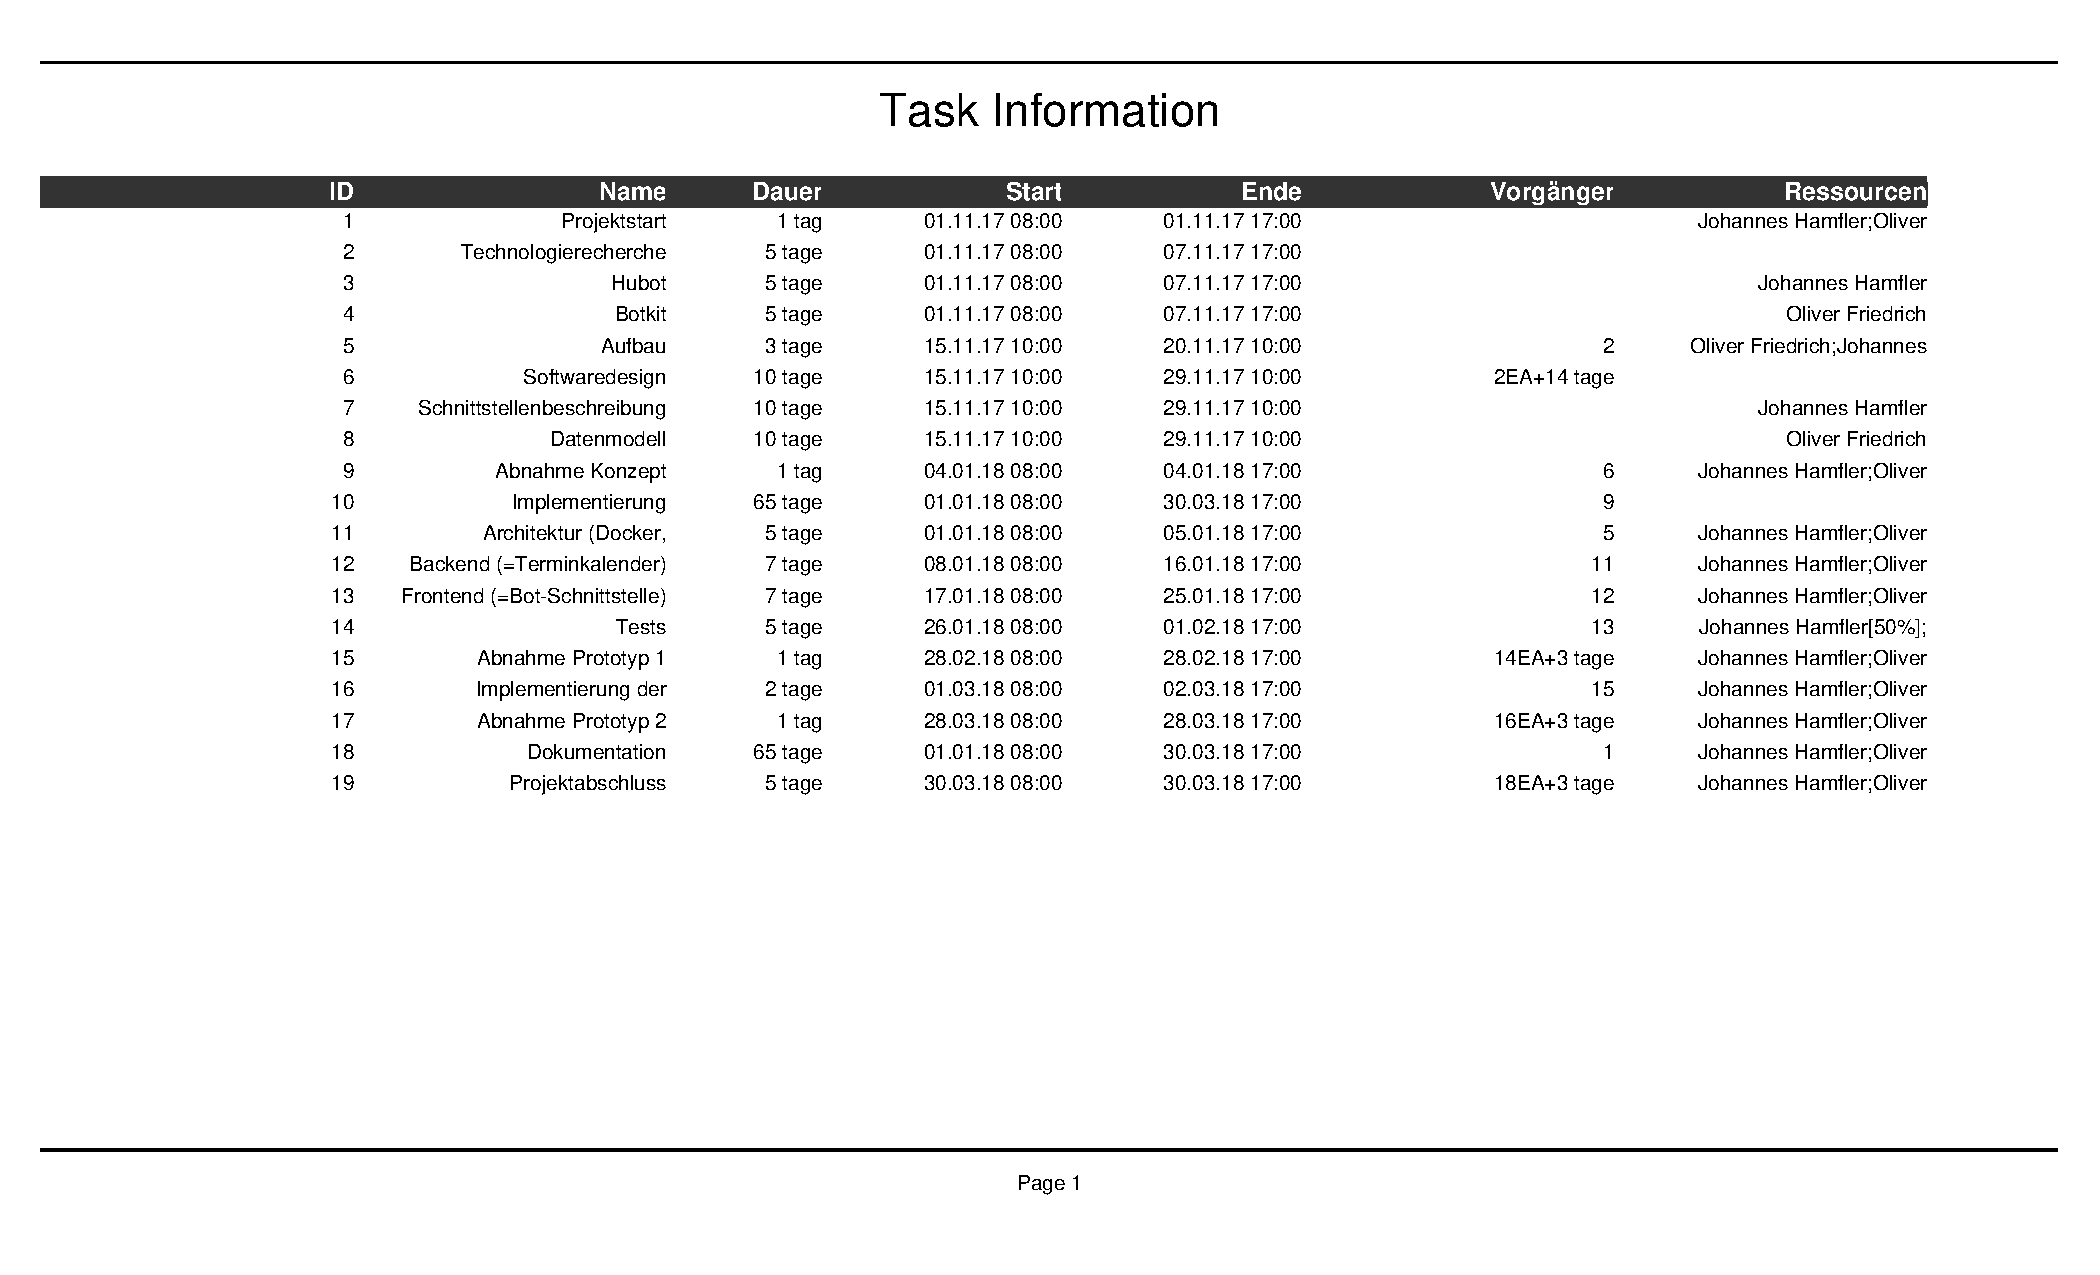
\includepdf[fitpaper]{../docs/Steckerbot_taskinfo.pdf}
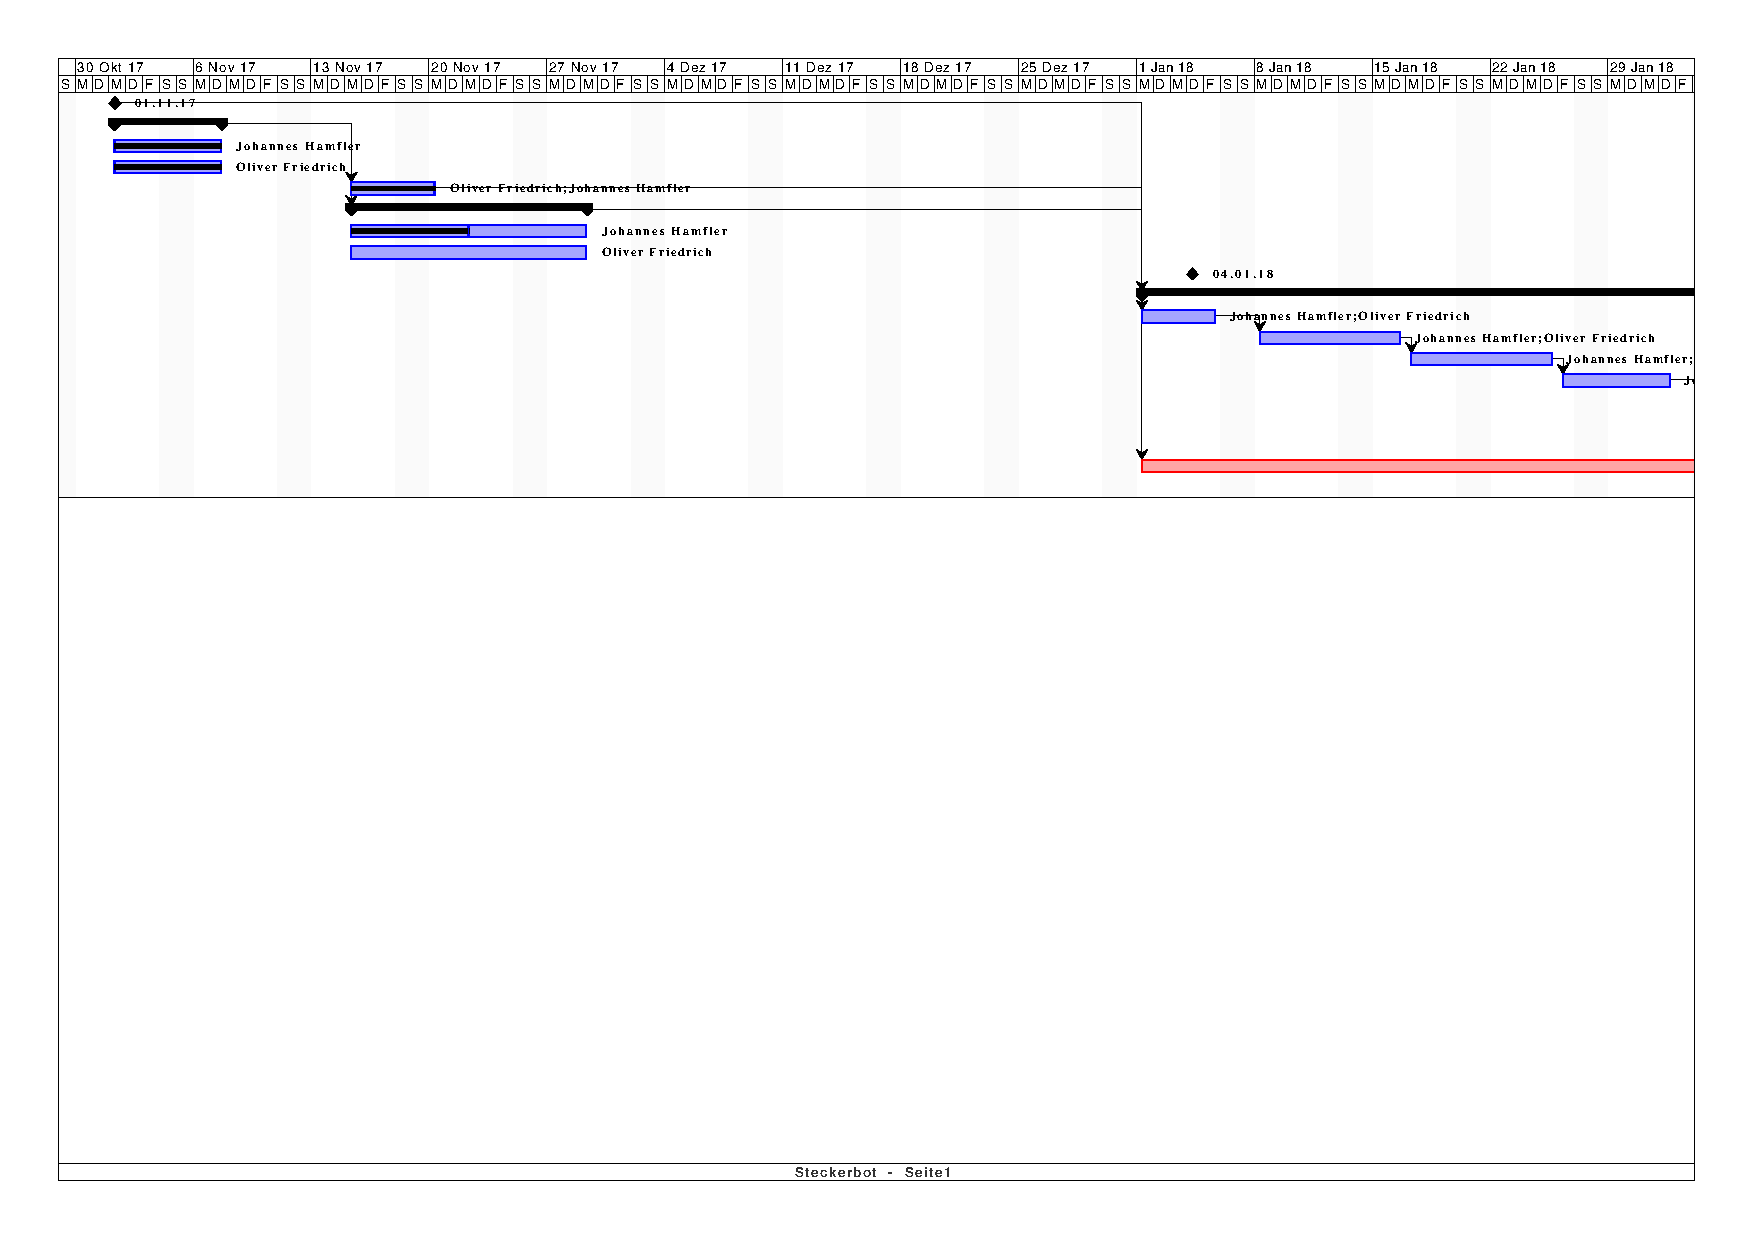
\includepdf[fitpaper]{../docs/Steckerbot_ganttchart.pdf}

\end{appendices}
